\documentclass{article}%
\usepackage[T1]{fontenc}%
\usepackage[utf8]{inputenc}%
\usepackage{lmodern}%
\usepackage{textcomp}%
\usepackage{lastpage}%
\usepackage[head=40pt,margin=0.5in,bottom=0.6in]{geometry}%
\usepackage{graphicx}%
%
\title{\textbf{DD HH de la UCAB: Carnet de la patria es una mutación de la lista Tascón}}%
\author{El Nacional Web}%
\date{04/10/2018}%
%
\begin{document}%
\normalsize%
\maketitle%
\textbf{URL: }%
http://www.el{-}nacional.com/noticias/politica/ucab{-}carnet{-}patria{-}una{-}mutacion{-}lista{-}tascon\_254344\newline%
%
\textbf{Periodico: }%
EN, %
ID: %
254344, %
Seccion: %
Política\newline%
%
\textbf{Palabras Claves: }%
Política, Mundo, Gobierno\newline%
%
\textbf{Derecho: }%
5%
, Otros Derechos: %
18%
, Sub Derechos: %
NO\_TIENE%
\newline%
%
\textbf{EP: }%
NO\newline%
\newline%
%
\textbf{\textit{El representante del organismo detalló, durante la audiencia de la CIDH, que realizaron informes en donde se evidencia "la evolución de la discriminación por motivos políticos"~}}%
\newline%
\newline%
%
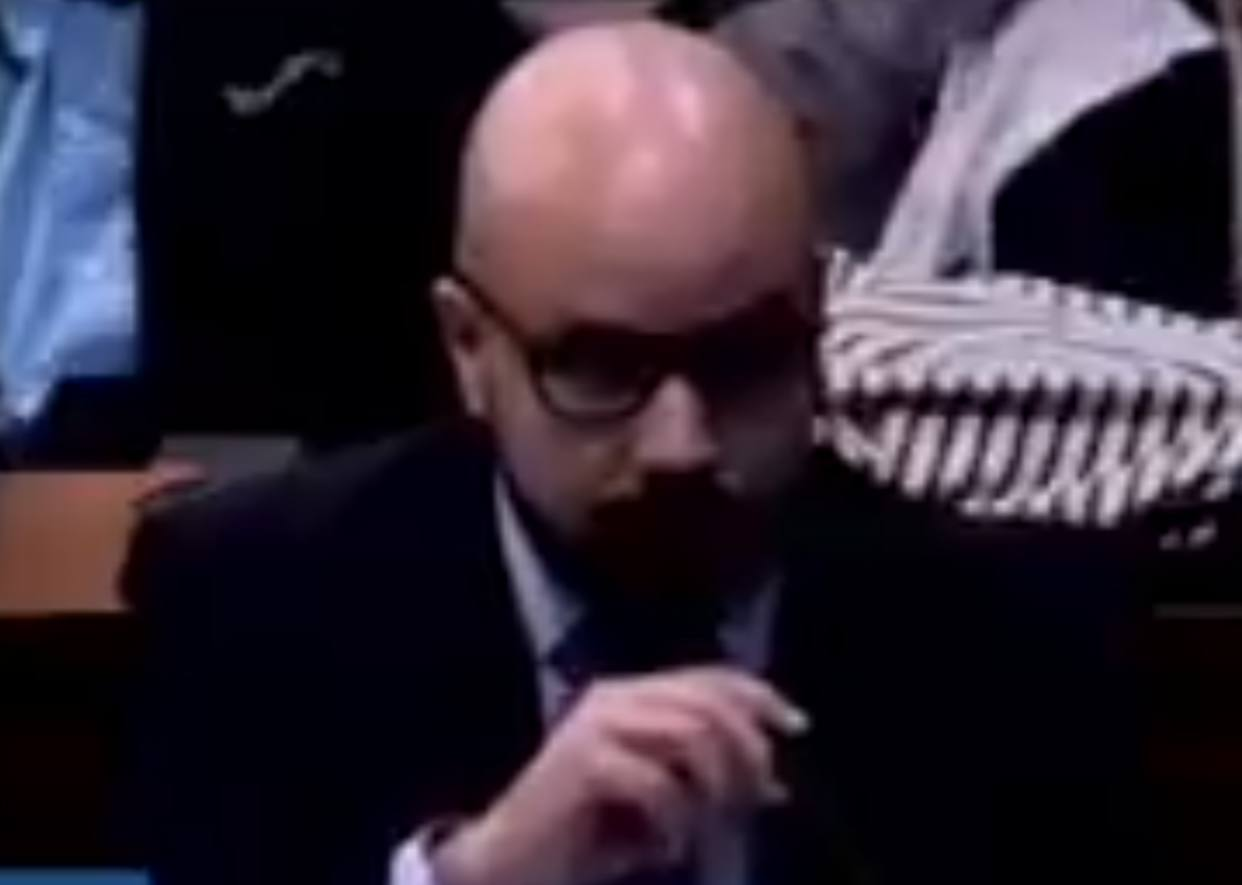
\includegraphics[width=300px]{209.jpg}%
\newline%
%
Eduardo Trujillo, representante del Centro de Derechos Humanos de la Universidad Católica Andrés Bello, indicó que el carnet de la patria es “una mutación de la lista Tascón”.%
\newline%
%
“La CIDH emitió una sentencia en el caso San Miguel y otros en relación a la denominada lista Tascón. En aquel fallo se puso de manifiesto la implementación del desvío de poder como una forma de discriminación. El carnet de la patria no es más que una mutación de la lista Tascón como un formato de discriminación en Venezuela”, dijo Trujillo durante su~ intervención en la audiencia de la Comisión Interamericana de Derechos Humanos (CIDH).%
\newline%
%
El representante señaló que el Centro de Derechos Humanos de la UCAB realizó diversos informes en los que~se demostró “la evolución de la discriminación por motivos políticos".%
\newline%
%
“Resulta claro cómo este instrumento de identificación es utilizado no exclusivamente para generar una discriminación positiva. Su efecto atenta contra el derecho a la igualdad, lo que a su vez tiene un efecto cascada en derechos civiles, políticos, económicos, culturales y sociales”, resaltó Trujillo.%
\newline%
%
\end{document}